\documentclass[
]{beamer}

\usepackage[czech]{babel}
\usepackage[utf8]{inputenc}
\usepackage[T1]{fontenc}
\usepackage{booktabs}
\usetheme[
  workplace=fi,
]{MU}

% Packages
\usepackage{tikz}

\begin{document}

\title{Adaptabilní systém pro výuku programování}
\subtitle{Program rektora}
\author[T.\,Effenberger]{Tomáš Effenberger\\ 410350@mail.muni.cz}
\institute[FI MU]{Fakulta informatiky Masarykovy univerzity}
\date{\today}
\subject{Předmět prezentace}
\keywords{klíčová, slova, prezentace}

\begin{frame}[plain]
\maketitle
\end{frame}

%\begin{frame}{Osnova}
%\tableofcontents
%\end{frame}

\begin{frame}{Výuka programování}
% Mise, rozsah, optimalni obtiznost, flow, blokove programovani.
% Existujici systemy (HoC) a pridana hodnota (vyzkum adaptability).
% Stav (2. prototyp), testovani na skolach.
\begin{figure}
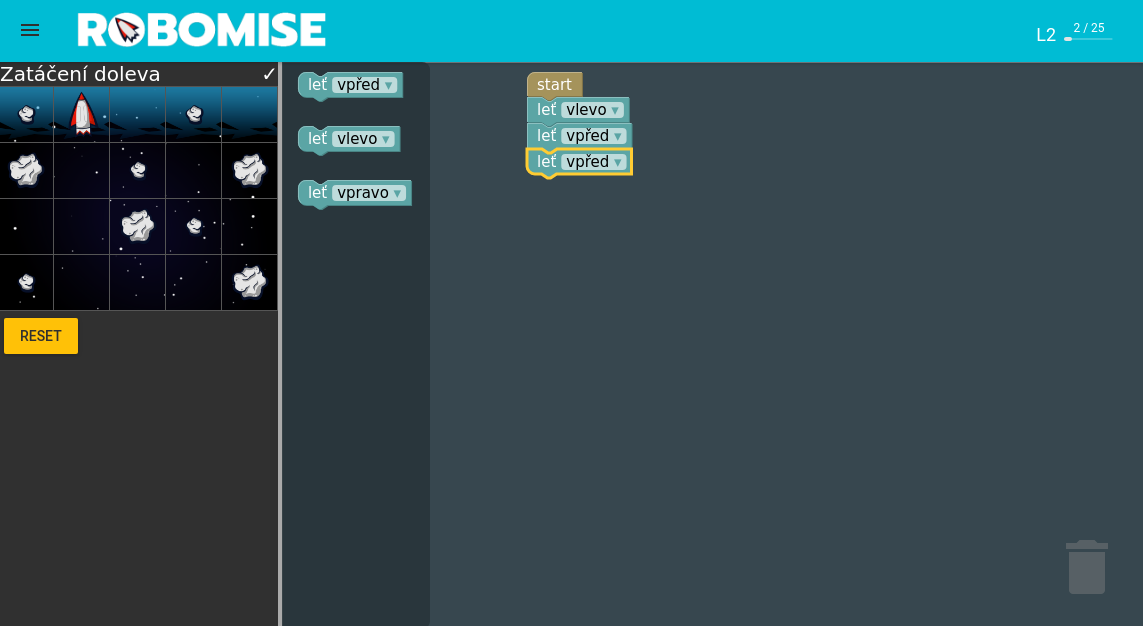
\includegraphics[width=\textwidth,height=.75\textheight,keepaspectratio]{../img/robomission-task1}
\end{figure}
\end{frame}

\begin{frame}{Programovací bloky}
% Proc: odstraneni problemu se syntaxi.
% Bloky: prikazy, cykly, podminky; kontrola barev a pozice.
\begin{figure}
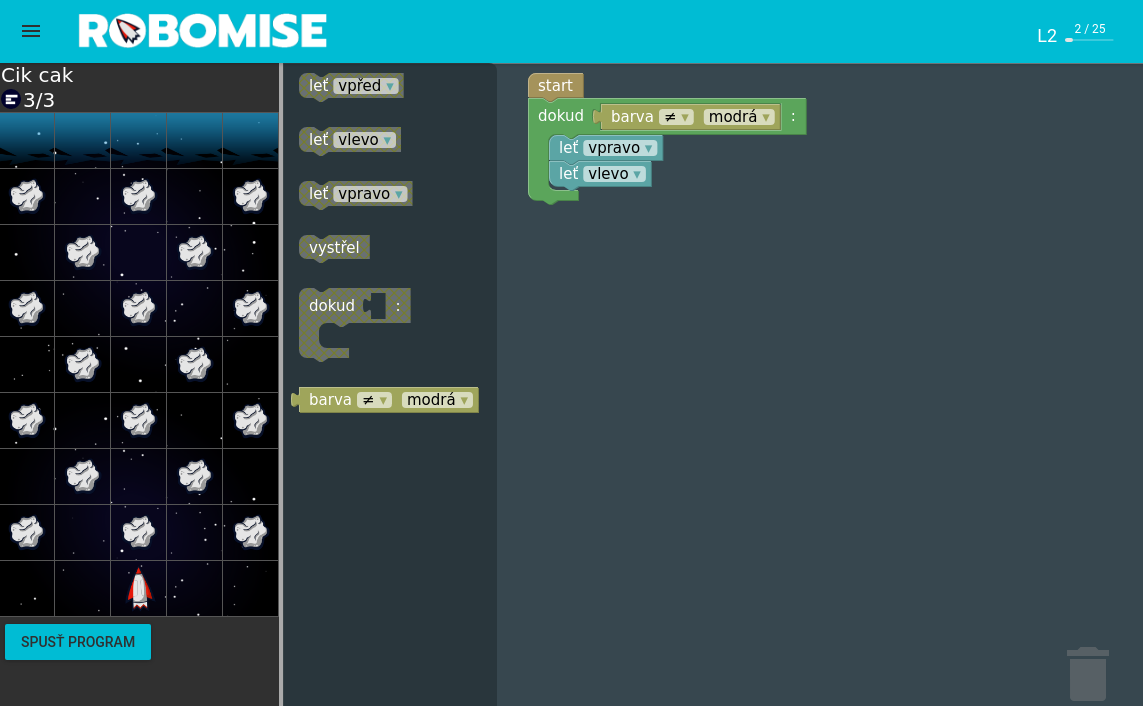
\includegraphics[width=\textwidth,height=.75\textheight,keepaspectratio]{../img/robomission-task2}
\end{figure}
\end{frame}

\begin{frame}{Herní prvky}
% Navrh hry: musi bavit a umoznovat rozpeti obtiznosti.
% robot na mrizce, staly let vpred, vice zakladnich akci.
% Herni prvky: diamanty, asteroidy, meteorodiy, cervi diry, barvy.
\begin{figure}
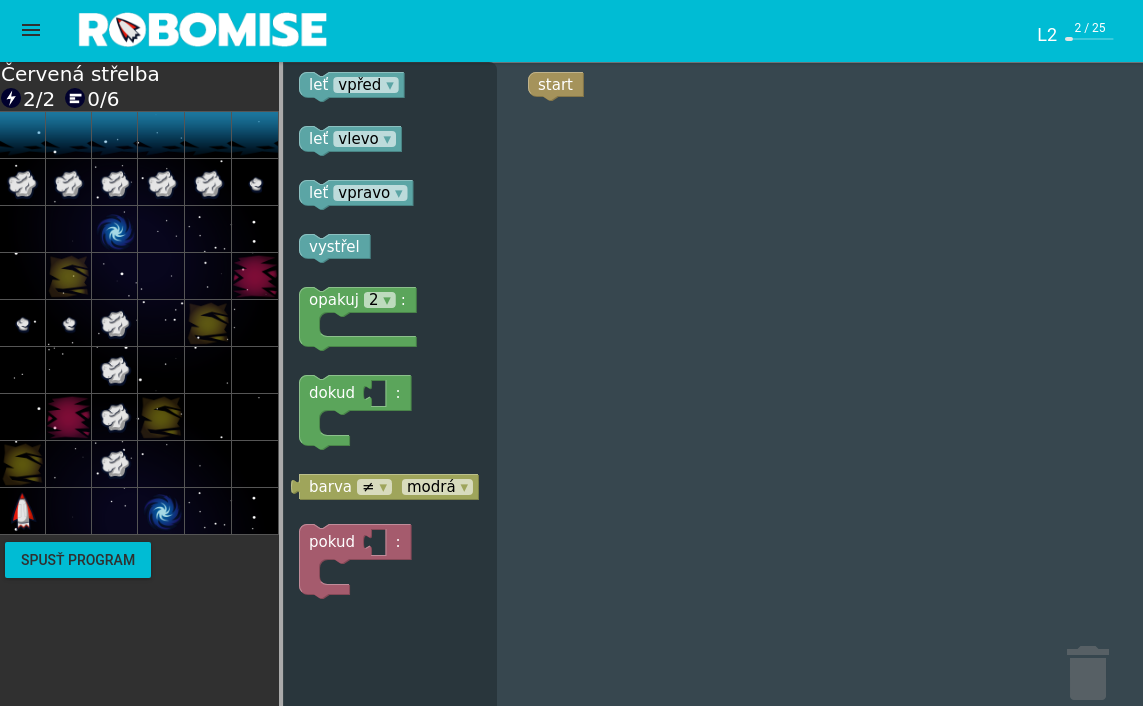
\includegraphics[width=\textwidth,height=.75\textheight,keepaspectratio]{../img/robomission-task3}
\end{figure}
\end{frame}

\begin{frame}{Adaptabilní instrukce}
% Adaptabilni instrukce a mini-vysvetleni.
\begin{figure}
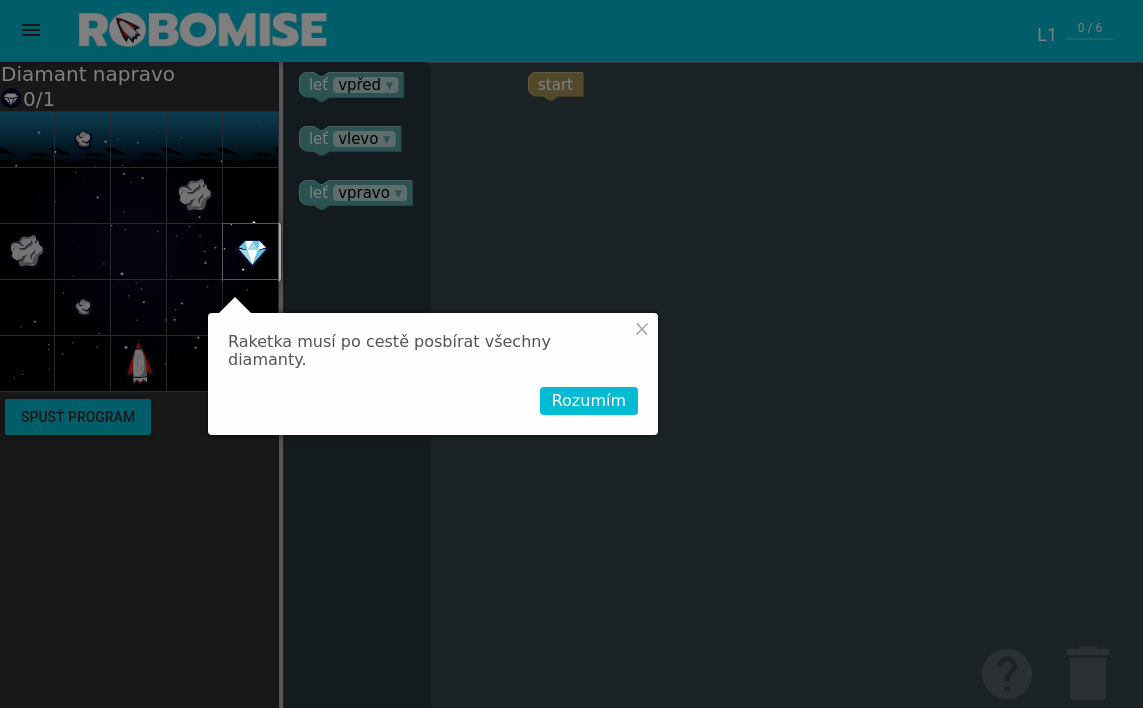
\includegraphics[width=\textwidth,height=.75\textheight,keepaspectratio]{../img/robomission-mini-instruction}
\end{figure}
\end{frame}

\begin{frame}{Levely a kredity}
% Motivacni prvky: kredity, levely.
% Aktualni verze je dost ad-hoc, uz brzy: mastery learning.
%\vspace{-10pt}
\begin{figure}
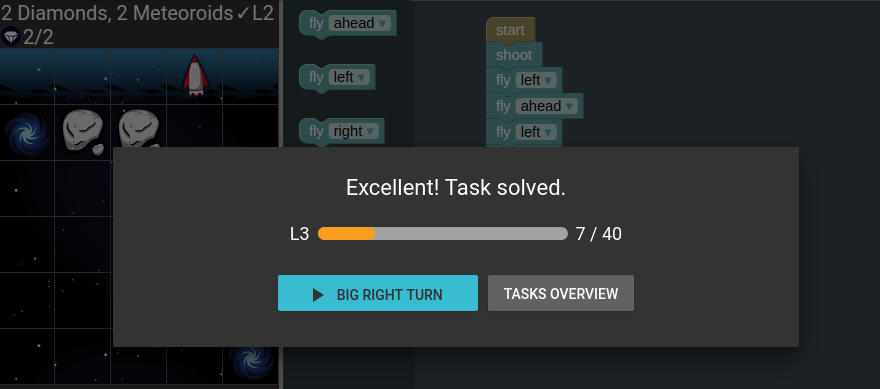
\includegraphics[width=0.9\textwidth,height=.75\textheight,keepaspectratio]{../img/robomission-levels-credits}
\end{figure}
\end{frame}

\begin{frame}{Přehled úloh}
% Pres 80 uloh, rozdelenych do 9 levelu.
\begin{figure}
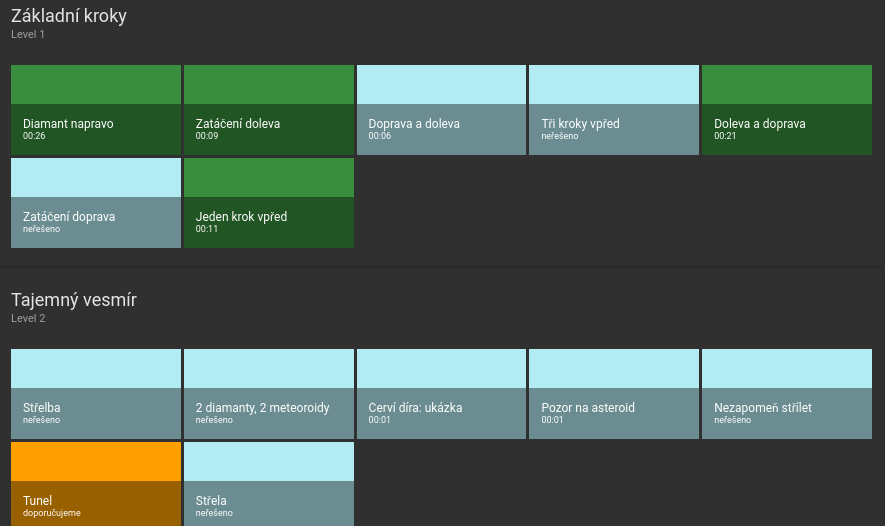
\includegraphics[width=\textwidth,height=.75\textheight,keepaspectratio]{../img/robomission-tasks-overview}
\end{figure}
\end{frame}

\begin{frame}{Doporučování úloh}
% Doporuceni uloh (jednoducha heuristika), predmet vyzkumu a aktualnich zmen.
% Snaha o optimalni obtiznost -> flow.
\begin{figure}
\begin{tikzpicture}[font=\sffamily,xscale=5, yscale=5]
\large
%\draw [lightgray, fill=gray] (0,0) -- (0.1,0) -- (1,0.8) -- (0.8,1) -- (0,0.1) -- (0,0);
\draw (0.1,0) -- (1,0.8);
\draw (0,0.1) -- (0.8,1);
\draw [thick, <->] (0,1) node [left] {obtížnost} -- (0,0) -- (1,0) node [below right] {dovednost};
\node at (0.27,0.82) {frustrace};
\node at (0.6,0.6) {flow};
\node at (0.7,0.2) {nuda};
\end{tikzpicture}
\end{figure}
\end{frame}

\begin{frame}{Anglická lokalizace}
\begin{figure}
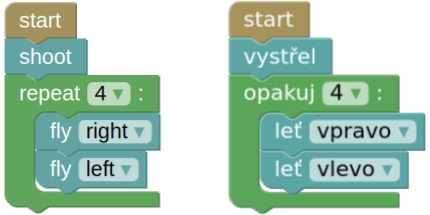
\includegraphics[width=0.5\textwidth,height=.75\textheight,keepaspectratio]{../img/roboblocks-english-czech}
\end{figure}
\end{frame}

\begin{frame}{Editor úloh}
% Online editor úloh. Moznost psat reseni v Pythonu a editovat mrizku ve vimu.
% Textovy format (markdown).
\begin{figure}
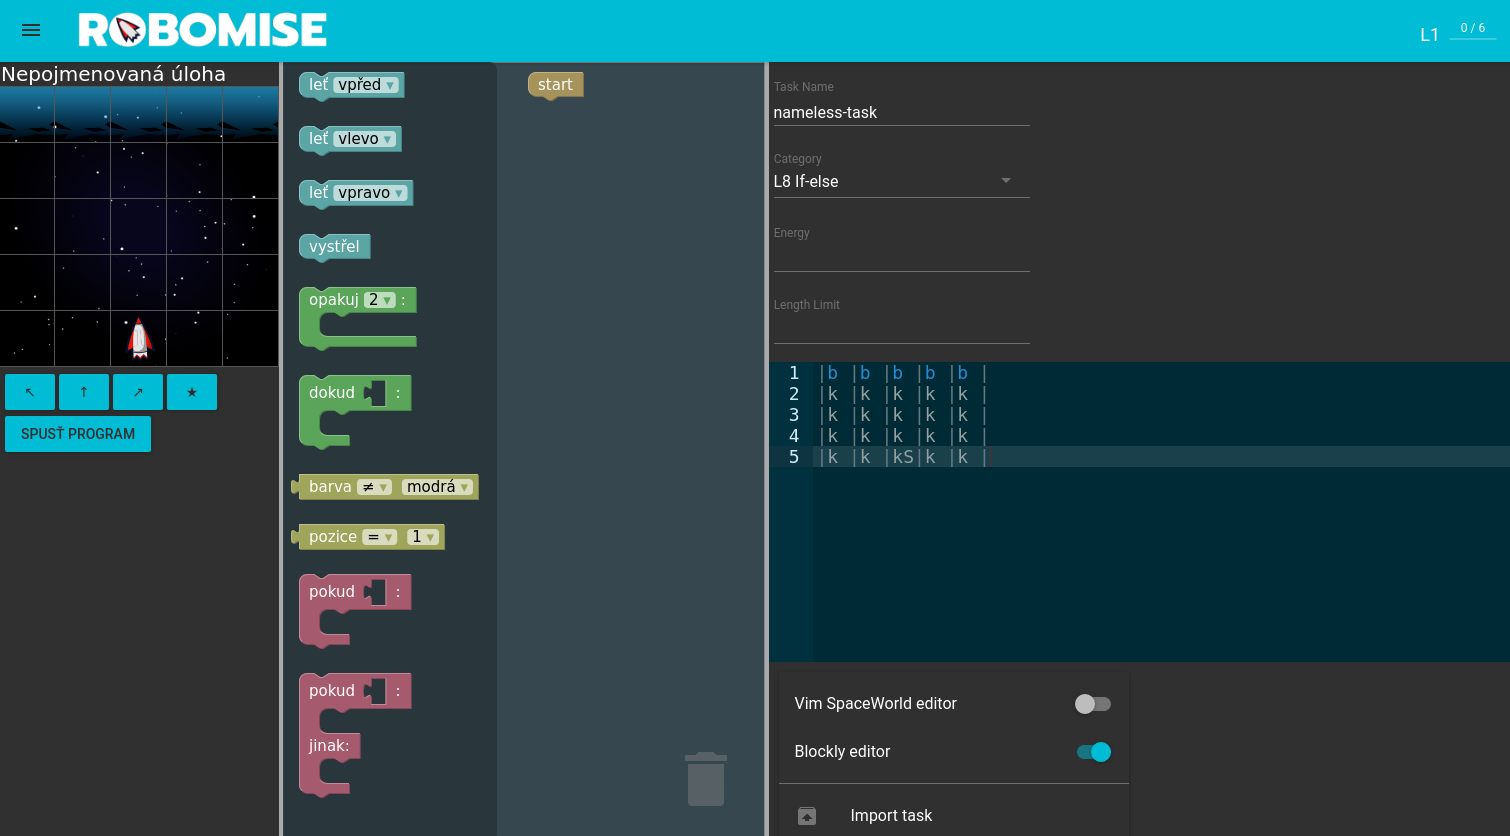
\includegraphics[width=\textwidth,height=.75\textheight,keepaspectratio]{../img/task-editor}
\end{figure}
\end{frame}

\begin{frame}{Monitoring}
% Google Analytics.
% Monitorovaci nastenka - metriky (napocitavane kazdy noc).
% Tydne updatovany jupyter notebook -- pohodlne rozsirovani.
\begin{figure}
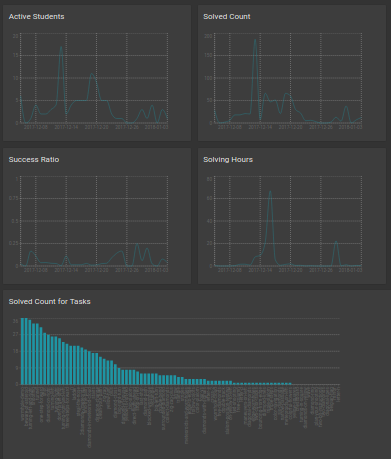
\includegraphics[width=0.44\textwidth]{../img/monitoring-dashboard}
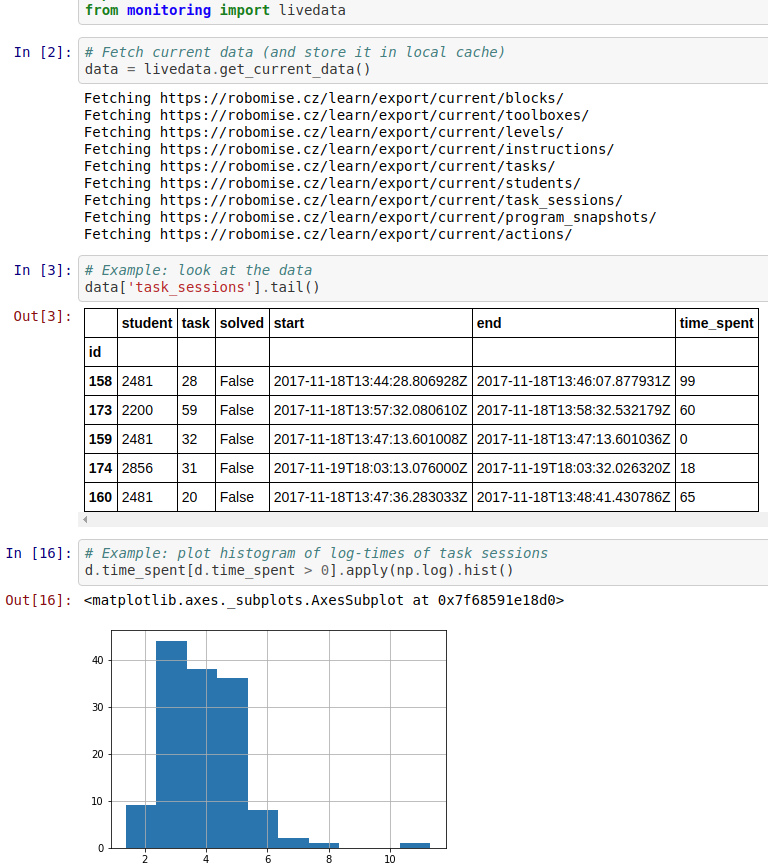
\includegraphics[width=0.45\textwidth]{../img/investigation-notebook}
\end{figure}
\end{frame}

\begin{frame}{Počet vyřešených úloh denně}
% Jednoduchý příklad sledované metriky - počet vyřešených úloh denně.
\begin{figure}
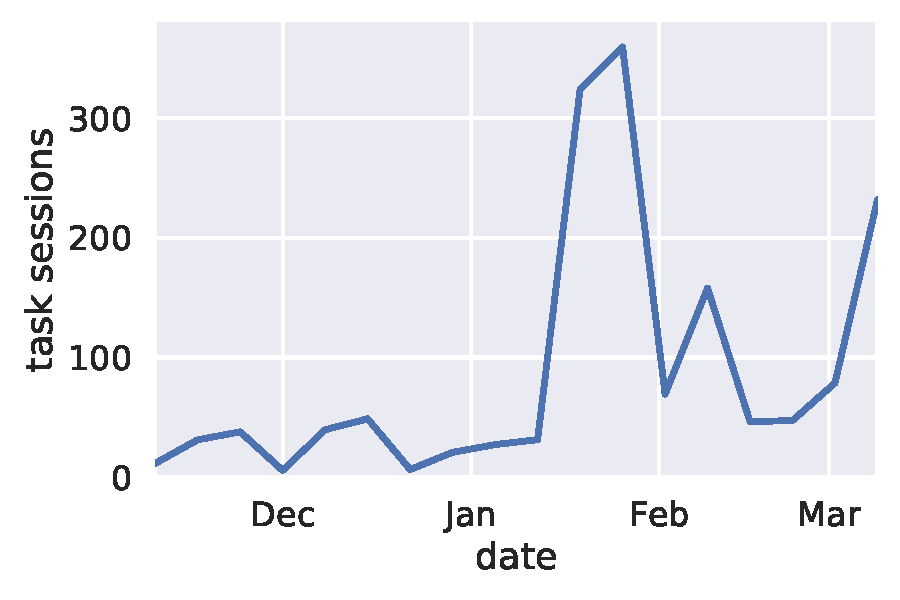
\includegraphics[width=0.8\textwidth]{../img/daily-task-sessions}
\end{figure}
\end{frame}

\begin{frame}{Obtížnost levelů}
% Ukazka analyzy: obtiznost levelu povetsinou roste, ale 7. je tezsi nez 8,
% indikace problemu (jsou tam trikove ulohy na testovani pozice).
% Graf navic ukazuje, ze distribuce casu je zhruba log-normalni.
\begin{figure}
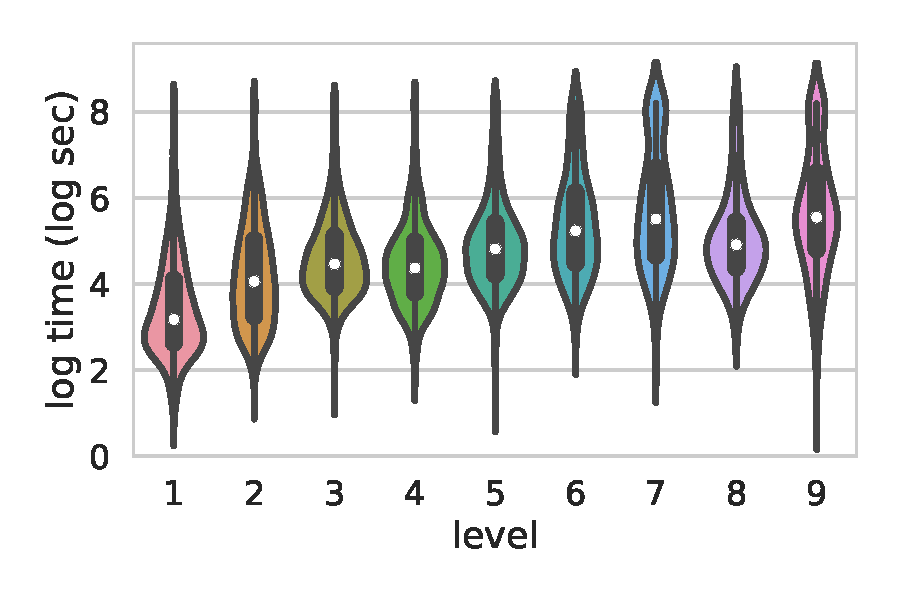
\includegraphics[width=0.8\textwidth]{../img/levels-time}
\end{figure}
\end{frame}

\begin{frame}{Shrnutí}
\begin{itemize}
\item adaptabilní systém pro výuku programování
\item úlohy na mřížce, blokové programování
\item optimální obtížnost úloh $\rightarrow$ flow
\item prototyp: \url{https://robomise.cz}
\item kód: \url{github.com/adaptive-learning/robomission}
\end{itemize}
\end{frame}


%\section[Název sekce 1]{Dlouhý název sekce 1}
%\subsection[Název podsekce 1]{Dlouhý název podsekce 1}

%\begin{frame}{Nadpis}{Podnadpis}
%běžný text, \structure{struktura stránky}, \alert{zvýrazněný text}
%\begin{itemize}
%  \item položka odrážkového seznamu na jeden řádek
%  \item položka odrážkového seznamu dlouhá, moc dlouhá (to aby se zalomila),
%    která navíc obsahuje \alert{zvýrazněný text}
%\end{itemize}
%\begin{enumerate}
%  \item a číslovaná odrážka
%  \begin{enumerate}
%    \item odrážka druhé úrovně se vzorečkem
%      \[ E = mc^2 \]
%  \end{enumerate}
%\end{enumerate}
%\end{frame}


%\begin{frame}{Textové bloky}
%text nad blokem
%\begin{block}{Blok}
%  text
%\end{block}
%\begin{exampleblock}{Blok s příkladem}
%  text
%\end{exampleblock}
%\begin{alertblock}{Zvýrazněný blok}
%  text
%\end{alertblock}
%\end{frame}

%\begin{frame}{Obrázky}
%\begin{figure}
%  \includegraphics[width=.5\textwidth,height=.5\textheight,keepaspectratio]{cow-black.mps}
%  \caption{Kráva černostrakatého holštýnského skotu}
%\end{figure}
%\end{frame}

%\begin{frame}{Tabulky}
%\begin{table}
%\begin{tabular}{llc}
%  Jméno & Příjmení & Rok narození \\ \midrule
%  Albert & Einstein & 1879 \\
%  Marie & Curie & 1867 \\
%  Thomas & Edison & 1847 \\
%\end{tabular}
%\end{table}
%\end{frame}

%\begin{frame}[plain]
%% Prostor na otazky.
%\vfill
%\centerline{Děkuji za pozornost.}
%\vfill\vfill
%\end{frame}

\end{document}
